\documentclass[dvipdfmx,autodetect-engine]{jsarticle}
\usepackage{tikz}
\usepackage[utf8]{inputenc}

\usepackage{amsmath,amssymb}
\usepackage{bm}
\usepackage{graphicx}
\usepackage{amsthm}
\usepackage{ascmac}
\usepackage{algorithm}
\usepackage{algorithmic}

\newcommand{\divergence}{\mathrm{div}\,}  %ダイバージェンス
\newcommand{\grad}{\mathrm{grad}\,}  %グラディエント
\newcommand{\rot}{\mathrm{rot}\,}  %ローテーション
\newtheorem{thm}{定理}[section]
\newtheorem{lem}[thm]{補題}
\newtheorem{axm}[thm]{公理}
\newcommand{\Axmref}[1]{公理\ref{#1}}
\newcommand{\Equref}[1]{式(\ref{equ:#1})}
\newcommand{\Conref}[1]{条件(\ref{equ:#1})}
\newcommand{\mbf}[1]{\mbox{\boldmath $#1$}}
\newcommand{\ave}[1]{\langle{#1}\rangle}
\newcommand{\itemb}[2]{\begin{itembox}[l]{#1}$#2$\end{itembox}}
\newcommand{\ov}[1]{\overline{#1}}
\newcommand{\eq}[1]{ \begin{equation}#1 \end{equation}}

\title{線形計画法}
\author{近藤 華 }
\date{July 2019}

\begin{document}

\maketitle

\section{線形計画法とは?}
以下の特徴を持つものを\textbf{線形計画}と呼ぶ.
\begin{itembox}[l]{線形計画}
\begin{itemize}
  \item n個の変数$x_{1},\cdots,x_{n}$は全て\textbf{非負}である.
  \item m個の制約条件は変数$x_{1},\cdots,x_{n}$の\textbf{1次式の不等式}(これを\textbf{制約不等式}と呼ぶ)である.
  \item 最大化する関数$f$(これを目的関数と呼ぶ)は変数$x_{1},\cdots,x_{n}$の\textbf{一次関数}である.
  \end{itemize}
\end{itembox}
特に,以下の問題P0のように表したものを線形計画の\textbf{標準形}という.
\begin{itembox}[l]{問題 P0}
\eq{
\label{equ:1}
	\left\{\begin{array}{ccccccccc}
	 	a_{11}x_{1} & +  & a_{12}x_{2} & + & \cdots &+ &  a_{1n}x_{n}  & \leq &b_{1}\\
     	 a_{21}x_{1} & + & a_{22}x_{2} & + & \cdots & + &  a_{2n}x_{n}  & \leq &b_{2}\\
    	\vdots &  & \vdots & & \ddots & & \vdots & &\vdots \\
      	a_{m1}x_{1} & + &a_{m2}x_{2} & +&\cdots & + &a_{mn}x_{n} & \leq & b_{m}\\
      \end{array}\right
    }
    \eq{
    \label{equ:2}
    x_{1} \geq 0, \hspace{15pt}  x_{2} \geq 0, \hspace{15pt}\cdots, \hspace{15pt} x_{n} \geq 0 
}
\eq{
	f  = c_{1}x_{1} + c_{2}x_{2} + \cdots +  c_{n}x_{n}  \to max
}
\end{itembox}
線形計画を解く手法を\textbf{線形計画法}(\textbf{リニアプログラミング})という.

\section{可能領域}
n次元空間内で\Conref{1},\Conref{2}の不等式を満たす点($x_{1},\cdots,x_{n}$)の集合を\textbf{可能領域}(\textbf{許容領域})といい,それに属する点($x_{1},\cdots,x_{n}$)を\textbf{可能解}(\textbf{許容解})という.可能解の中で目的関数を最大にする点($x_{1}$*$,\cdots,x_{n}$*)を\textbf{最適解}という.
\begin{itembox}[l]{定理1}
(問題 P0に最適解が存在する時)問題 P0の可能領域はn次元空間内の凸多面体である.
\end{itembox}
-定理の証明用空欄-
\\
\\
\\
\\
\\
\\
\\
\\
\\
\\

\section{線形計画の基本定理}
\begin{itembox}[l]{定理2}
問題 P0の最適解($x_{1}$*$,\cdots,x_{n}$*)が存在すれば,目的関数は可能領域の頂点で最大値をとる.
\end{itembox}
-定理の証明空欄-
\\
\\
\\
\\
\\
\\
\\
\\
\\
\\

\begin{itembox}[l]{定理3}
問題 P0のある最適解($x_{1}$*$,\cdots,x_{n}$*)において,\Conref{1},\Conref{2}の$m+n$個の不等式のうち$n$個が等号で成立する.
\end{itembox}

上記のことから,問題 P0は,'原理的'に次のようにして解くことができる.

\begin{enumerate}
\item \Conref{1},\Conref{2}の$m+n$個の不等式のうちから$n$個を選んで等号に置き換えた連立一次方程式を解く.
\item その解が非負であって,残りの制約不等式を満たすか調べる.
\item 満たせば目的関数$f$の値を計算する.
\item これを全ての可能性について行い,$f$の値が最大になるものを選ぶ.
\end{enumerate}

けれど,少し考えればこの$n$個の選び方は組合せ$\left(\begin{array}{c}m+n\\n\end{array}\right)$の数だけあることがわかる.よってこれは実際的ではない.

\section{スラック変数}
不等式は\textbf{小さい方の辺}に非負の数を加えて等式にすることができる.
例:$a + b \leq 0 \iff a + b + \lambda = 0 ~~ただし,\lambda \geq 0$
上の例のように不等式の小さい方の辺に付け加える非負の変数のことを\textbf{スラック変数}と呼ぶ.問題 P0にスラック変数$\lambda_{1},\cdots\lambda_{m}$を導入すると,問題 P0は問題 P1のように表すことができる.
\begin{itembox}[l]{問題 P1}
\eq{
\label{equ:3}
	\left\{\begin{array}{ccccccccccc}
	 	a_{11}x_{1} & +  & a_{12}x_{2} & + & \cdots &+ &  a_{1n}x_{n} & + & \lambda_{1} & = &b_{1}\\
     	 a_{21}x_{1} & + & a_{22}x_{2} & + & \cdots & + &  a_{2n}x_{n}  &+ & \lambda_{2} & = &b_{2}\\
    	\vdots &  & \vdots & & \ddots & & \vdots & & \vdots & &\vdots \\
      	a_{m1}x_{1} & + &a_{m2}x_{2} & +&\cdots & + &a_{mn}x_{n} & + & \lambda_{m} & = & b_{m}\\
      \end{array}\right
    }
    \eq{
    \label{equ:4}
    x_{1} \geq 0, \hspace{15pt}  x_{2} \geq 0, \hspace{15pt}\cdots, \hspace{15pt} x_{n} \geq 0 
}
\eq{
    \label{equ:4}
    \lambda_{1} \geq 0, \hspace{15pt}  \lambda_{2} \geq 0, \hspace{15pt}\cdots, \hspace{15pt} \lambda_{m} \geq 0 
}
\eq{
	f  = c_{1}x_{1} + c_{2}x_{2} + \cdots +  c_{n}x_{n}  \to max
}
\end{itembox}
 スラック変数$\lambda_{1},\cdots\lambda_{m}$は,\Conref{1}の制約不等式において,\textbf{左辺が右辺よりどれだけ小さいか}を示す量である.したがって,$\lambda_{i}=0$と言うことは\Conref{1}の$i$番目の制約不等式が\textbf{等号で成立している}ということ.これを幾何学的に解釈すれば\textbf{n次元空間の可能領域の$i$番目の境界面で$\lambda_{i}=0$である}と言える.よって解は,この平面上または$\lambda_{i}<0$側の半空間になければならない.
  また,定理$6.3$について問題 P1について書き直すと以下のようになる.
\begin{itembox}[l]{定理4}
問題 P0のある最適解($x_{1}$*$,\cdots,x_{n}$*,$\lambda_{1},\cdots\lambda_{m}$)において,$m+n$個の値$x_{1}$*$,\cdots,x_{n}$*,$\lambda_{1},\cdots\lambda_{m}$のうちの$n$個は0である.
\end{itembox}
上記のことから,問題 P0は,'原理的'に次のようにして解くことができる.

\begin{enumerate}
\item $m+n$個の変数のうちから$n$個を選んで0と置いてできる連立一次方程式\ref{3}を残りの$m$個の変数について解く.
\item その解が全て非負かどうか調べる.
\item そうであれば目的関数$f$の値を計算する.
\item これを全ての可能性について行い,$f$の値が最大になるものを選ぶ.
\end{enumerate}

$m+n$個の変数のうちから$n$個を選んで0と置く変数のことを\textbf{非基底変数},残りの$m$個の変数を\textbf{基底変数},n個の非基底変数を0と置くことによって得られる解を\textbf{基底解}と呼ぶ.
ただこの方法もn個の非基底変数を選ぶ選び方が$\left(\begin{array}{c}m+n\\n\end{array} \right) $ 通りあり,実際的ではない.そこで\textbf{シンプレックス法}が考え出された.

\section{シンプレックス法}
選んだ$n$個の非基底変数から一つを排除し,別の変数を新たに0とするような「変数の交換」(ただし目的関数が\textbf{必ず増加するように}変数を選ぶ)を次々と行う方法である.

実際に例題を解いてみよう.
見やすいように,$\lambda_{1},\lambda_{2}$は$x_{3},x_{4}$と表している.
\begin{itembox}[l]{例題 1}
\eq{
\label{equ:5}
	\left\{\begin{array}{cccccccc}
	 	2x_{1} & +  & 8x_{2} & + &  a_{1n}x_{3} & & = & 60\\
     	4x_{1} & +  & 4x_{2} & + &  &a_{1n}x_{4}& = & 60\\
      \end{array}\right
    }
    \eq{
    \label{equ:6}
    x_{1} \geq 0, \hspace{15pt}  x_{2}  \geq 0,  \hspace{15pt}x_{3}  \hspace{15pt} \geq 0, x_{4} \geq 0
}
\eq{
	f  = 29x_{1} + 45x_{2} \to max
}
\end{itembox}

-解き方(板書するので自分で書いてください.)-
\\
\\
\\
\\
\\
\\
\\
\\
\\
\\
\\
\\
\\
\\
\\
\\
\\
\\
\\
\\
\\
\\
\\
\\
\\
\\
\\

念の為,シンプレックス法が終了した時に得られる解が最適解であることを確認しておく.
シンプレックス法の方法より得られた解である頂点に隣接する全ての頂点では,$f$ は等しいか小さくなっている.よってもし,得られた解が最適解でないとしたら,可能領域が凹を含んだ多面体でなければあり得ない.しかし最適解が存在する時,可能領域は凸多面体である.よって,得られた解は最適解.


シンプレックス法が終了した時,毎回$f$が増加する限り次のどちらかになる.
\begin{enumerate}
\item 最適解に到達している.このことは\textbf{全ての$c_{j}$}が\textbf{0または負}になっていることで判定できる.
\item $f$が発散して最適解が存在しない.このことは$f$の係数$c_{j}$が正となる変数があり,制約式の中で\textbf{その変数の係数$a_{ij}$が全て非負}になることで判定できる.
\end{enumerate}
そのほかの可能性として以下の2つがある.
\begin{enumerate}
\item 出発する非負の解が見つからない.
\item 変数の交換を行っても$f$の値が変化しない.
\end{enumerate}
1. の場合は,単に見つかりにくい場合と可能領域が空集合の場合,そもそも非負の解が存在しない場合がある.これは\textbf{人口変数}によって解決する.2.の場合は\textbf{退化}と呼ばれる現象である.

\section{退化}
 n次元空間内の可能領域を表す多面体の頂点は$n$枚の境界面の交わりとして定義されるが,たまたまそこで$n+1$枚以上の平面が交わっていることもある.この時,シンプレックス法の途中で変数を交換しても\textbf{$f$の値は変化しない}ということが起きる.どの変数を右に持っていくかという解釈は変わってくるのだけれども.これを\textbf{退化}(又は\textbf{縮退})という.

 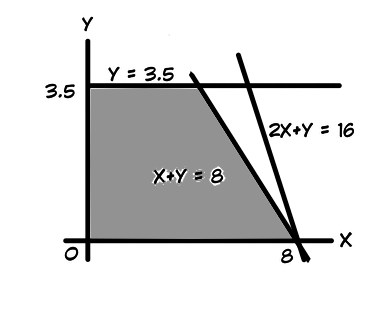
\includegraphics[width=6cm]{degeneration_0}  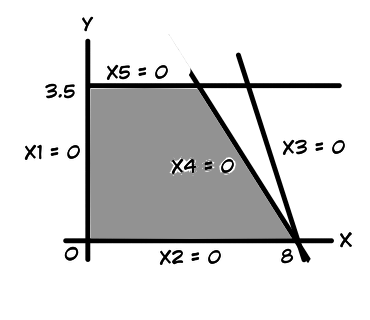
\includegraphics[width=6cm]{degeneration_1}
 
 
\section{人口変数}
問題 P0の標準形をしていなくても変形によって標準形に帰着する場合がある.
\begin{itemize}
\item 変数の中に非負はなく,$x_{i}\leq 0$の条件があれば,全ての$x_{i}$を$-x_{i}$で置き換えて,$x_{i}\geq 0$ の条件に変える.
\item 制約不等式の中に不等号の向きが反対の形の\eq{a_{i1}x_{1}+\cdots+a_{in}x_{n}\geq b_{i}}のものがあれば,両辺に-1を掛けて次のように不等号の向きを変える.\eq{\label{equ:8}-a_{i1}x_{1}-\cdots-a_{in}x_{n}\leq -b_{i}}
\item 制約条件の中に等式の形の\eq{a_{i1}x_{1}+\cdots+a_{in}x_{n}= b_{i}}のものがあれば,これを2つの不等式に置き換える.\eq{a_{i1}x_{1}+\cdots+a_{in}x_{n}\geq b_{i}} \eq{a_{i1}x_{1}+\cdots+a_{in}x_{n}\leq b_{i}}後者は上に示したように,両辺に-1をかけることによって\Equref{8}のようにかける.
\item 目的関数を最大にするのではなく,\eq{
	f  = c_{1}x_{1} + c_{2}x_{2} + \cdots +  c_{n}x_{n}  \to min
}のように宰相にするのなら,両辺に-1を掛けて,$f'=-f$と置くと,$f'$の最大化になる.\eq{
	f'(=-f) = -c_{1}x_{1} - c_{2}x_{2} - \cdots -  c_{n}x_{n}  \to max
}
\end{itemize}

シンプレックス方では最初に非負の解が見つからなければ次に進めないが,上記のように変換を行うと出発する解が見つけにくいことがある.そのような時の対策の一つとして\textbf{人口変数}の導入がある.

\begin{itembox}[l]{例題6.16}
次の線形計画を解け.\\
\eq{
\label{equ:9}
	\left\{\begin{array}{ccccccccccc}
	 	x &- &0.5y &\geq& 1\\
     	x &-&y&\leq &2\\
    	x&+&y&\leq &4\\
      \end{array}\right
      }
 \eq{ x \geq 0, \hspace{15pt} y \geq 0}
 \eq{f=2x+y\to max}
\end{itembox}
(解)
\begin{enumerate}
\item 第一の不等式の向きが反対なので直す.
\item $x_{1}=x,x_{2}=y$と置き,スラック変数$x_{3},x_{4},x_{5}$を導入する.
\item 右辺に$x_{1}とx_{2}$が残るように式変形すると,\eq{
	\begin{array}{ccccccc}
	 	x_{3} &= &-1 &+ &x_{1} &-&0.5x_{2} \\
     	x_{4} &=&2&- &x_{1}&+&x_{2}\\
    	x_{5}&=&4&- &x_{1}&-&x_{2}\\
    	f&=&&&2x_{1}&+&x_{2}\\
      \end{array}\\
      }\\となり,解は\eq{x_{1} = 0, \hspace{15pt}x_{2} = 0, \hspace{15pt}x_{3} = -2, \hspace{15pt}x_{4} = 2, \hspace{15pt}x_{5} = 4,\hspace{15pt}f = 0}となる.
\item ところが,$x_{3}$が負なのでこの値から出発することはできない.そこで新しい変数$x_{6}$を付け加えて,\eq{x_{3}=-1+x_{1}-0.5x_{2}+x_{6}, \hspace{15pt}x_{6}\geq 0}としてみる.
\item これを$x_{6}$について解くと,\eq{\label{equ:10}x_{6}=1-x_{1}+0.5x_{2}+x_{3}}となり都合が良い.しかし,問題が変わってしまう.しかし最終的な最適解で$x_{6}=0$となっていれば問題は変わったことにはならない.よって,目的関数$f$に$-Mx_{6}$という項を付け加えることで最適解で$x_{6}=0$となるように強制する.ただし$M$は非常に大きい数.\eq{\hat{f}=f-Mx_{6}=2x_{1}&+&x_{2}-Mx_{6}}この$x_{6}$ような変数を人口変数(又は人為変数)と呼ぶ.
\item \Equref{10}をこの$\hat{f}$の式に代入して$x_{6}$を消去する.
\item 前と同じようにしてとくと,最終的に\eq{
	\begin{array}{ccccccccc}
	 	x_{1} &= &3 &- &0.5x_{4} &-&0.5x_{5}& &\\
     	x_{3} &=&1.5&- &0.75x_{4}&-&0.25x_{5}&+&x_{6}\\
    	x_{2}&=&1&+ &0.5x_{4}&-&0.5x_{5}& & \\
    	f&=&7&-&0.5x_{4}&-&1.5x_{5}&-&Mx_{6}\\
      \end{array}\\
      }\\となり,次の最適解を得る.\eq{x_{1} = 3, \hspace{15pt}x_{2} = 1, \hspace{15pt}x_{3} = 1.5, \hspace{15pt}x_{4} = 0, \hspace{15pt}x_{5} = 0,\hspace{15pt}x_{6}=,0\hspace{15pt}\hat{f} = 7}
\end{enmerate}

人口変数を用いると,常に非負の解が作れるので,たとえ可能領域が空集合であって,非負の解が存在しない場合でも\textbf{非負の解が人口的に}作れてしまう.
まとめると,人口変数を用いて非負の解を人口的に作ってシンプレックス法を適用すると,次の3通りのどれかになる.
\begin{itemize}
\item 発散して,最適解が存在しない.
\item 最適解に到達して,人口変数は全て0となる.
\item 最適解に到達するが,人口変数の中には0にならないものがある.
\end{itemize}
最後の場合が,可能領域が空集合の場合にあたる.よってこれを利用すれば与えられた\textbf{可能領域が空集合かどうか}を判定することができるぞ.
\\ \\
双対変数までやりたかったが,多分解説が終わらないので次の人に任せる.

\end{document}
